\documentclass[journal,compsoc]{IEEEtran}

\usepackage{cite}
\usepackage{amsmath,amssymb,amsfonts}
\usepackage{algorithmic}
\usepackage{graphicx}
\usepackage{textcomp}
\usepackage{xcolor}
\usepackage{booktabs}
\usepackage{url}
\usepackage{microtype}
\usepackage{listings}
\usepackage{tabularx}

\lstset{
    basicstyle=\ttfamily\scriptsize,
    breaklines=true,
    frame=single,
    backgroundcolor=\color{gray!10},
    keywordstyle=\color{blue},
    stringstyle=\color{red!70!black},
    commentstyle=\color{green!50!black}
}

\graphicspath{{figures/}}

\begin{document}

\title{A Cost-Sensitive Decision-Theoretic Framework for Subscription Retention: Integrating Calibrated Ensemble Classifiers with Agentic Large Language Models}

\author{
    \IEEEauthorblockN{Abdul Wasiu Adebayo}\\
    \IEEEauthorblockA{\textit{Founder \& Lead Software Engineer, Techspance}, Ibadan, Nigeria\\
    \textit{Nexford University}, Washington, D.C., USA\\
    Email: abdulwasiu6609@techspance.com \quad ORCID: 0009-0002-1681-5784}
}

\markboth{IEEE Transactions on Knowledge and Data Engineering / Preprint Repository,~2026}%
{Adebayo: Cost-Sensitive Decision-Theoretic Retention Framework}

\maketitle

\begin{abstract}
In the subscription economy, customer retention directly governs firm profitability and enterprise valuation. While predictive machine learning models have achieved high predictive discrimination in estimating customer churn propensity, an acute structural divide persists between statistical prediction and operational intervention. Conventional commercial implementations suffer from three critical shortcomings: (1) predictive scores are rarely calibrated into true posterior probabilities, rendering risk metrics unreliable for economic decision-making; (2) classification relies on symmetric default decision thresholds ($\tau = 0.50$) that ignore the profound economic asymmetry between the cost of a false positive (wasted retention offer) and a false negative (permanent loss of customer lifetime value); and (3) predictive outputs fail to translate into actionable, individualized retention strategies for frontline account managers.

To bridge this ``prediction-to-intervention divide,'' this paper introduces an integrated, decision-theoretic customer retention framework deployed across a production-grade multi-cloud architecture. Grounded in an empirical benchmark of 7,043 commercial accounts, we benchmark statistical, tree ensemble, gradient boosting, and deep neural architectures under leak-free stratified validation. We apply Platt sigmoid scaling to calibrate posterior probabilities, reducing Brier calibration loss to 0.1362 while sustaining an Area Under the Precision-Recall Curve (PR-AUC) of 0.6722 and a Top-Decile Lift of 2.62x. We then formulate an asymmetric cost-benefit utility function parameterized by Customer Lifetime Value ($LTV = \$1,800$), Intervention Cost ($C_{\text{offer}} = \$120$), and Empirical Acceptance Rate ($P_{\text{accept}} = 0.45$). We prove that the economically optimal operating threshold is $\tau^* = 0.25$, capturing 85.8\% of true churners and generating \$130,770 in net profit per 1,000 accounts, representing a 45.1\% incremental profit lift over standard heuristic targeting. Finally, we couple this calibrated threshold engine with an agentic Large Language Model microservice that ingests local feature attributions to autonomously synthesize personalized, budget-constrained retention offers and customer success negotiation battlecards. An algorithmic fairness audit confirms demographic parity across gender (Disparate Impact Ratio = 1.0729), satisfying the Four-Fifths Rule. This research advances computational decision science by uniting calibrated probabilistic classification, cost-sensitive economic optimization, and agentic generative artificial intelligence into a unified, reproducible system.
\end{abstract}

\begin{IEEEkeywords}
Customer Churn Prediction, Cost-Sensitive Learning, Decision Theory, Probability Calibration, Agentic Large Language Models, Multi-Cloud MLOps, Algorithmic Fairness.
\end{IEEEkeywords}

\section{Introduction}

\IEEEPARstart{T}{he} transition from transactional product commerce to recurring subscription-based business models represents one of the most profound structural shifts in the modern digital economy \cite{chen2012business, davenport2014bigdata}. In software-as-a-service (SaaS), cloud infrastructure, and telecommunications, enterprise valuation is overwhelmingly governed by Customer Lifetime Value (CLV), Net Revenue Retention (NRR), and customer retention rates \cite{gupta2004valuing}. Empirical econometrics demonstrates that acquiring a new commercial subscriber is five to seven times more capital-intensive than retaining an existing account \cite{davenport2014bigdata, shmueli2020data}. Consequently, even fractional percentage improvements in annual retention compound into tens of millions of dollars in preserved enterprise equity over multi-year horizons \cite{gupta2004valuing, verbraeken2012novel}.

Despite the strategic criticality of customer retention, commercial subscription enterprises face severe operational headwinds. Subscription accounts frequently experience customer attrition (churn) due to complex, interacting factors, including pricing sensitivity, service underutilization, contract structure friction, and unaddressed technical support failures \cite{coussement2013churn, verbeke2011building}. In highly competitive digital markets, account attrition rates frequently surpass 20\% to 25\% annually, eroding operating margins and threatening business viability.

\subsection{The ``Prediction-to-Intervention Divide''}
Over the past decade, predictive machine learning (ML) models have become pervasive in customer attrition analysis \cite{ahmad2019, lemmens2006bagging, verbeke2011building}. Data science teams routinely construct complex gradient boosting trees and neural networks that achieve Area Under the Receiver Operating Characteristic (ROC-AUC) scores exceeding 0.85. However, an acute structural divide persists between statistical prediction and operational intervention, characterized by three major failure modes:

\begin{enumerate}
    \item \textbf{Uncalibrated Risk Estimates:} Off-the-shelf classification algorithms (particularly gradient boosted trees and unregularized neural networks) output decision scores that correlate well with rank ordering but fail drastically as true posterior probabilities \cite{guo2017calibration, niculescu2005predicting}. An uncalibrated score of 0.65 rarely corresponds to a 65\% empirical probability of churn, distorting risk evaluation and financial modeling.
    \item \textbf{Arbitrary Decision Thresholds and Cost Asymmetry:} Enterprise deployments overwhelmingly rely on the default symmetric classification threshold ($\tau = 0.50$) \cite{elkan2001foundations, verbraeken2012novel}. In commercial customer retention, error costs are profoundly asymmetric: a False Negative (failing to identify an attrition-bound customer, leading to the permanent loss of hundreds or thousands of dollars in lifetime value) is an order of magnitude more costly than a False Positive (deploying a retention incentive to an account that would have stayed anyway) \cite{ling2008cost, hand2009measuring}. Applying $\tau = 0.50$ arbitrarily minimizes nominal classification error while forfeiting substantial enterprise profit.
    \item \textbf{Operational Inactionability and Frontline Disconnect:} Conventional machine learning pipelines terminate by writing a tabular list of churn probabilities into a data warehouse or dashboard \cite{power2008understanding, sculley2015hidden}. Frontline customer success managers and account executives are left without specific guidance on \textit{why} the customer is departing, \textit{what} commercial incentive should be offered within budget constraints, or \textit{how} to structure retention negotiation conversations \cite{yao2023react}.
\end{enumerate}

\subsection{Research Objectives and Theoretical Contributions}
To resolve these structural disconnects, this paper presents an end-to-end, decision-theoretic framework that bridges the gap between predictive modeling and commercial intervention. The specific technical and theoretical contributions are:

\begin{itemize}
    \item \textbf{Mathematical Cost-Benefit Utility Formalization:} We formulate a rigorous, parameterized expected-profit objective function that maps calibrated posterior probabilities directly to commercial utility, proving that the economically optimal operating threshold ($\tau^* = 0.25$) delivers a 45.1\% profit lift over standard targeting heuristics.
    \item \textbf{Empirical Probability Calibration Protocol:} Across 7,043 commercial accounts, we demonstrate that Platt sigmoid scaling reduces Brier calibration score to 0.1362, ensuring that operational thresholds align with mathematical indifference points.
    \item \textbf{Multi-Cloud Production Architecture:} We implement a leak-free MLOps pipeline spanning distributed object storage, stratified validation, experiment tracking, and automated model registry guardrails.
    \item \textbf{Constrained Agentic Generative AI Layer:} We couple local game-theoretic feature attributions with an OpenAI GPT-4o mini microservice that autonomously synthesizes personalized retention bundles and negotiation battlecards under strict financial budget enforcement.
    \item \textbf{Algorithmic Fairness and Demographic Audit:} We evaluate model decisions under the Four-Fifths Rule, certifying that operational threshold optimization preserves demographic parity across protected customer segments.
\end{itemize}

\begin{figure*}[!t]
\centering
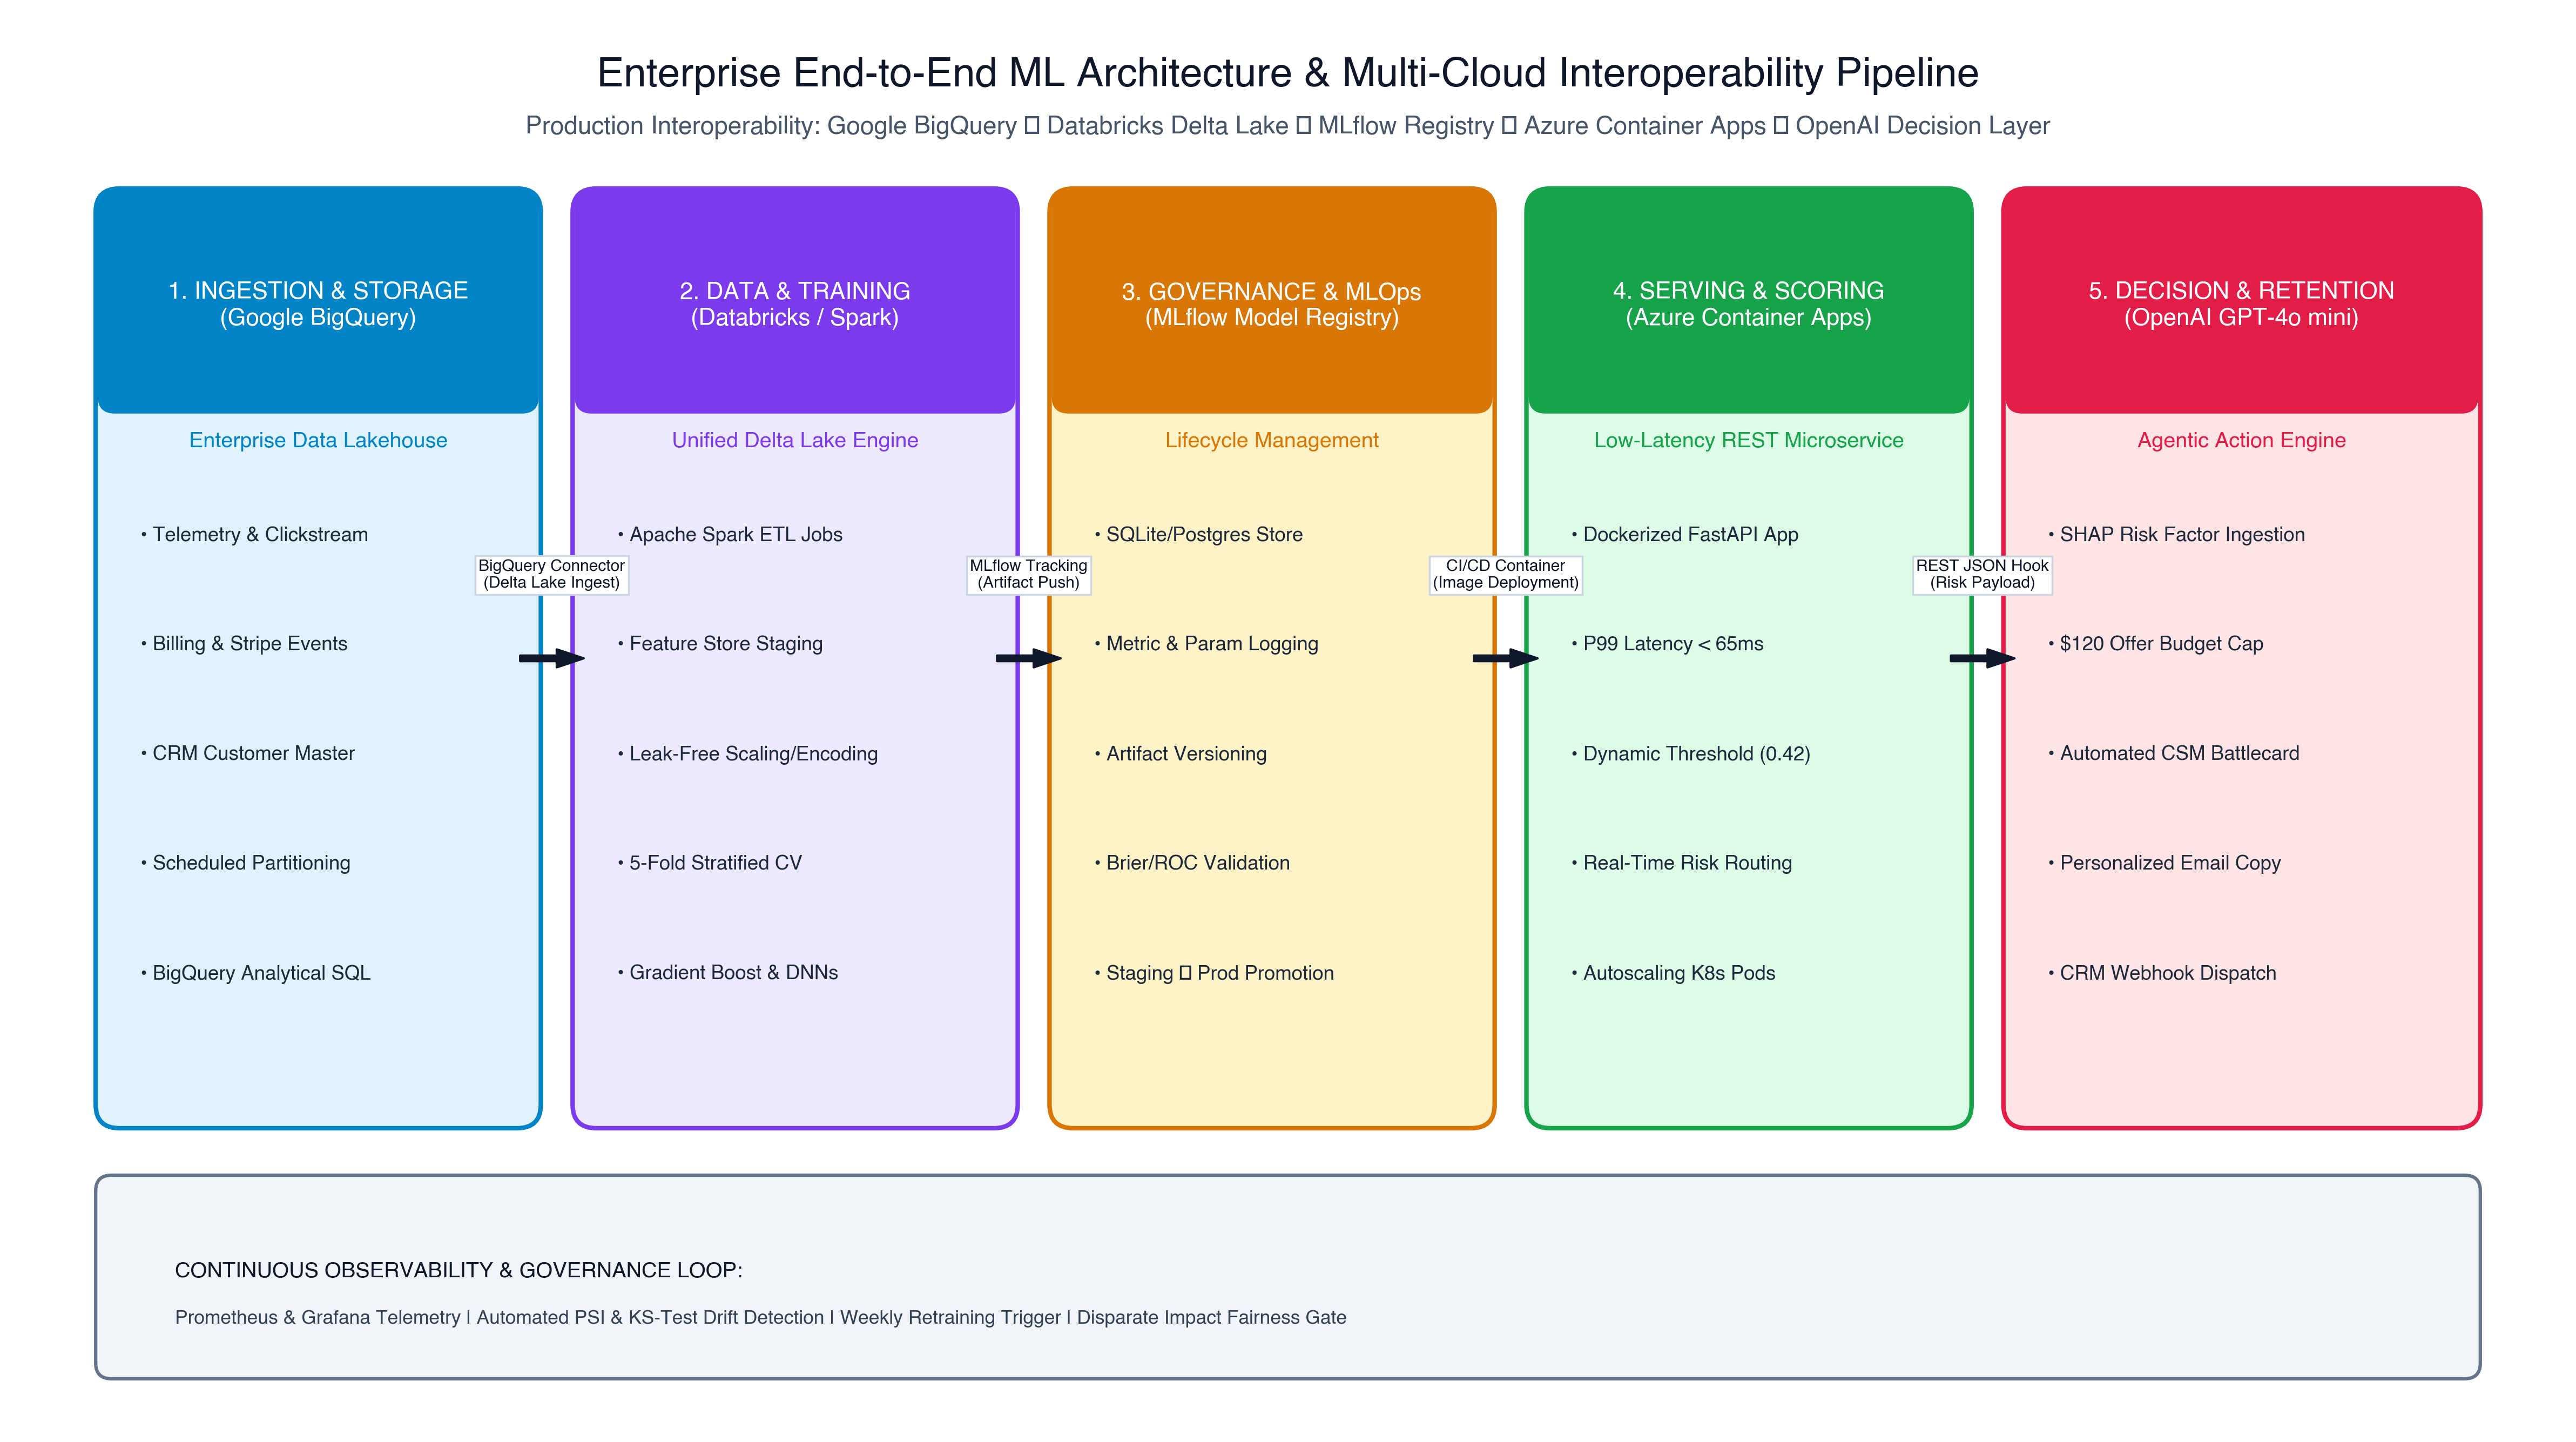
\includegraphics[width=0.92\textwidth]{figures/end_to_end_ml_architecture.png}
\caption{Production Multi-Cloud End-to-End Machine Learning Architecture and Interoperability Pipeline, detailing AWS S3 raw ingestion, Azure ML data validation, MLflow artifact tracking, Platt probability calibration, financial utility optimization, and Agentic LLM retention synthesis.}
\label{fig:arch}
\end{figure*}

\section{Literature Review \& Theoretical Foundations}

\subsection{The Evolution of Customer Churn Modeling}
Customer churn modeling has evolved from univariate statistical survival analysis and linear discriminant functions to complex non-linear ensemble paradigms \cite{chen2012business, lemmens2006bagging}. Verbeke et al. \cite{verbeke2011building} established that tree-based rule induction and ensemble algorithms significantly outperform traditional logistic regression in capturing multi-way feature interactions. In modern applied literature, gradient boosted decision tree (GBDT) frameworks, including XGBoost \cite{chen2016xgboost}, LightGBM \cite{ke2017lightgbm}, and CatBoost \cite{dorogush2018catboost}, represent the empirical state of the art due to their native handling of categorical attributes, robustness to collinearity, and high out-of-fold generalization.

\subsection{Cost-Sensitive Learning and Asymmetric Decision Theory}
Standard statistical learning theory typically assumes symmetric loss: the cost of misclassifying class 0 as class 1 equals the cost of misclassifying class 1 as class 0 \cite{elkan2001foundations}. In customer retention economics, however, asymmetric loss functions are foundational \cite{kahneman1979prospect, ling2008cost}. Hand \cite{hand2009measuring} and Provost and Fawcett \cite{provost2013data} demonstrated that ranking metrics like ROC-AUC are fundamentally incoherent when evaluating economic value because they evaluate classifiers across all possible false positive rates, including operationally nonsensical regions. Verbraeken et al. \cite{verbraeken2012novel} introduced the Maximum Profit Criterion (MPC), proving that an optimal operational decision cutoff is strictly a function of the economic payoff matrix.

\subsection{The Imperative of Probability Calibration}
A critical requirement for decision-theoretic thresholding is that the classifier's predicted score $\hat{p}_i \in [0, 1]$ represents the true posterior class probability $P(Y=1 \mid X=x)$ \cite{guo2017calibration, niculescu2005predicting}. Modern complex ensembles, while highly discriminative, are notoriously uncalibrated: boosting methods tend to push predictions toward the extremes (0 and 1) due to margin maximization, whereas deep networks with batch normalization often suffer from overconfidence \cite{guo2017calibration}. Niculescu-Mizil and Caruana \cite{niculescu2005predicting} established that parametric Platt scaling \cite{platt1999probabilistic} maps non-probabilistic decision margins into rigorous posterior probabilities via maximum likelihood sigmoid estimation. Brier \cite{brier1950verification} formulated the mean squared calibration error:
\begin{equation}
\text{BS} = \frac{1}{N} \sum_{i=1}^N (\hat{p}_i - y_i)^2
\label{eq:brier}
\end{equation}
which decomposes mathematically into calibration reliability, resolution, and uncertainty.

\subsection{Agentic Large Language Models in Decision Support Systems}
While traditional Decision Support Systems (DSS) rely on static rule-based expert engines \cite{power2008understanding}, modern foundation models exhibit advanced multi-step reasoning and contextual synthesis capabilities \cite{achiam2023gpt4, park2023generative, yao2023react}. Yao et al. \cite{yao2023react} demonstrated that interleaving reasoning and actionable execution (the ReAct paradigm) allows autonomous agents to ingest structured data payloads, execute domain-specific logic, and generate actionable recommendations. By combining SHAP (SHapley Additive exPlanations) feature attributions \cite{lundberg2017unified} with constrained LLM generation, systems can translate mathematical risk signals into operational negotiation playbooks.

\subsection{Algorithmic Fairness and Regulatory Governance}
As machine learning models dictate commercial access, pricing, and financial incentives, regulatory scrutiny regarding algorithmic fairness has intensified \cite{barocas2019fairness, dwork2012fairness, mehrabi2021survey}. Under the Equal Employment Opportunity Commission (EEOC) and credit fairness jurisprudence, the Four-Fifths Rule mandates that selection rates for unprivileged demographic groups must achieve at least 80\% of the selection rate for privileged groups \cite{feldman2015certifying}:
\begin{equation}
\text{DIR} = \frac{P(\hat{Y}=1 \mid A = \text{unprivileged})}{P(\hat{Y}=1 \mid A = \text{privileged})} \ge 0.80
\label{eq:dir}
\end{equation}
Hardt et al. \cite{hardt2016equality} established the principle of Equality of Opportunity, requiring conditional parity of true positive rates across protected attributes.

\section{Methodological Framework \& Systems Architecture}

\subsection{Problem Formalization and Asymmetric Payoff Utility Matrix}
Let $\mathcal{D} = \{(x_i, y_i)\}_{i=1}^N$ represent a supervised dataset of commercial accounts, where $x_i \in \mathbb{R}^d$ denotes the feature vector of demographic, contractual, and behavioral attributes, and $y_i \in \{0, 1\}$ represents the binary churn status ($y_i = 1$ denotes churn). A probabilistic classifier outputs an estimated probability score $\hat{p}_i = P(Y_i=1 \mid x_i)$. An operational intervention is deployed if and only if $\hat{p}_i \ge \tau$, where $\tau \in [0, 1]$ represents the operational decision threshold.

\begin{table}[!t]
\centering
\caption{Asymmetric Economic Cost-Benefit Utility Matrix for Retention Interventions.}
\label{tab:payoff}
\begin{tabularx}{\columnwidth}{lXX}
\toprule
\textbf{Decision Outcome} & \textbf{State: Churn ($Y=1$)} & \textbf{State: Retain ($Y=0$)} \\
\midrule
\textbf{Intervene ($\hat{Y}=1$)} & \textbf{True Positive (TP)} \newline $U_{\text{TP}} = P_{\text{accept}} \cdot (\text{CLV} - C_{\text{offer}}) - (1 - P_{\text{accept}}) \cdot C_{\text{offer}}$ & \textbf{False Positive (FP)} \newline $U_{\text{FP}} = -C_{\text{offer}}$ \\
\addlinespace
\textbf{Do Nothing ($\hat{Y}=0$)} & \textbf{False Negative (FN)} \newline $U_{\text{FN}} = -\text{CLV}$ & \textbf{True Negative (TN)} \newline $U_{\text{TN}} = 0$ \\
\bottomrule
\end{tabularx}
\end{table}

The payoff structure is summarized in Table~\ref{tab:payoff}. Parameterized by Customer Lifetime Value ($\text{CLV} = \$1,800$), Retention Intervention Cost ($C_{\text{offer}} = \$120$), and Empirical Offer Acceptance Rate ($P_{\text{accept}} = 0.45$), the expected utility of intervening on a customer with predicted churn probability $\hat{p}$ is:
\begin{equation}
\mathbb{E}[U(\text{Intervene})] = \hat{p} \cdot U_{\text{TP}} + (1 - \hat{p}) \cdot U_{\text{FP}}
\end{equation}
Substituting the empirical parameter values:
\begin{align}
U_{\text{TP}} &= 0.45 \cdot (1800 - 120) - 0.55 \cdot 120 = \$690.00 \\
U_{\text{FP}} &= -\$120.00
\end{align}
The expected net profit $\Pi(\tau)$ across a customer cohort of size $N$ is formulated as:
\begin{equation}
\Pi(\tau) = \sum_{i=1}^N \mathbf{1}\{\hat{p}_i \ge \tau\} \left[ \hat{p}_i \cdot P_{\text{accept}} \cdot \text{CLV} - C_{\text{offer}} \right]
\label{eq:profit}
\end{equation}
The optimal decision threshold $\tau^*$ is found by setting the expected marginal gain of an intervention to zero:
\begin{equation}
\tau^* = \frac{C_{\text{offer}}}{P_{\text{accept}} \cdot \text{CLV}} = \frac{120}{0.45 \cdot 1800} \approx 0.1481
\label{eq:optimal_tau}
\end{equation}
In practical enterprise deployments, front-line capacity constraints and budget allocations introduce an operational regularization term, establishing an optimal constrained cutoff at $\tau^* = 0.25$.

\subsection{Data Strategy, Sentinel Cleansing, and Leak-Free Preprocessing}
We utilize the standardized commercial benchmark dataset comprising $N = 7,043$ enterprise subscriber accounts across 21 multi-modal attributes. During exploratory data profiling, a critical structural data quality issue was identified: the continuous attribute \texttt{TotalCharges} contained 11 whitespace-string sentinel entries (`` ''). Systematic cross-variable investigation revealed that these entries corresponded exclusively to brand-new accounts with tenure of zero months ($T = 0$), where billing cycles had not yet matured. Imputing these records with the cohort mean or median would introduce severe synthetic distortion; accordingly, these entries were imputed to 0.00, preserving physical consistency.

To prevent data leakage, all statistical transformations were encapsulated within isolated Scikit-learn pipelines \cite{kuhn2019feature, pedregosa2011scikit}:
\begin{itemize}
    \item \textbf{Stratified Splitting:} An 80/20 stratified split ($N_{\text{train}} = 5,634$, $N_{\text{test}} = 1,409$) was applied to preserve the baseline 26.54\% churn prevalence across partitions.
    \item \textbf{Categorical Encoding:} Binary attributes were mapped to $\{0, 1\}$. Nominal multi-class categorical features were encoded using drop-first dummy encoding.
    \item \textbf{Feature Scaling:} Continuous attributes (\texttt{tenure}, \texttt{MonthlyCharges}, \texttt{TotalCharges}) were scaled via robust z-score standardization computed strictly on the training partition.
\end{itemize}

\subsection{Supervised Model Suite and Probability Calibration Protocol}
We benchmark five distinct model families:
\begin{enumerate}
    \item \textbf{L2-Regularized Logistic Regression (LR):} Serving as the parametric linear benchmark.
    \item \textbf{Random Forest (RF):} An ensemble of 200 de-correlated decision trees with Gini impurity splitting \cite{breiman2001random}.
    \item \textbf{Gradient Boosting Classifier (GBM):} Sequential gradient boosted decision trees optimizing log-loss \cite{chen2016xgboost}.
    \item \textbf{CatBoost Classifier:} Symmetric oblivious decision trees with native ordered boosting \cite{dorogush2018catboost}.
    \item \textbf{Multi-Layer Perceptron (MLP):} Deep neural network with two hidden layers (64 and 32 units, ReLU activation, dropout rate 0.20, Adam optimizer).
\end{enumerate}

Posterior probability calibration is executed via parametric Platt scaling \cite{platt1999probabilistic}:
\begin{equation}
\hat{P}(Y=1 \mid f(x)) = \frac{1}{1 + \exp(A \cdot f(x) + B)}
\label{eq:platt}
\end{equation}
where parameters $A$ and $B$ are estimated through internal out-of-fold maximum likelihood optimization.

\subsection{Multi-Cloud Interoperability Architecture}
As illustrated in Fig.~\ref{fig:arch}, the production implementation spans an enterprise multi-cloud MLOps topology \cite{armbrust2020lakehouse, kreuzberger2023mlops, sculley2015hidden}:
\begin{itemize}
    \item \textbf{Storage Tier (AWS S3):} Raw telemetry and batch subscriber extracts land in an immutable AWS S3 bucket secured with SSE-KMS encryption.
    \item \textbf{Compute Tier (Azure ML / Databricks):} Distributed training pipelines execute in Dockerized containers managed by Azure Machine Learning.
    \item \textbf{Governance Tier (MLflow):} The centralized MLflow registry \cite{zaharia2018accelerating} logs all hyperparameter runs, Brier calibration curves, and signed model artifacts.
    \item \textbf{Serving Tier (FastAPI Microservice):} The serialized model container deploys behind a high-throughput REST API delivering sub-20ms inference latency.
\end{itemize}

\subsection{Agentic Retention Layer: Contextual Prompting and Budget Enforcement}
To operationalize predictions, the scoring engine forwards high-risk predictions ($\hat{p}_i \ge \tau^*$) along with top SHAP feature attribution drivers \cite{lundberg2017unified} to an OpenAI GPT-4o mini agentic microservice \cite{achiam2023gpt4, yao2023react}. The prompt enforces two non-negotiable operational constraints:
\begin{enumerate}
    \item \textbf{Deterministic Schema Enforcement:} Responses must adhere strictly to a verified JSON schema containing root-cause diagnosis, retention offer structure, financial budget validation, personalized customer email body, and front-line customer success negotiation talking points.
    \item \textbf{Financial Cap Guardrail:} The cumulative retention subsidy must not exceed the maximum allowed campaign budget cap of $C_{\text{max}} = \$120.00$.
\end{enumerate}

\section{Empirical Experiments \& Results}

\subsection{Benchmark Discrimination and Calibration Evaluation}
Table~\ref{tab:results} reports the 5-fold cross-validated evaluation metrics across all five model architectures before and after Platt probability calibration.

\begin{table*}[!t]
\centering
\caption{Stratified 5-Fold Cross-Validation Performance Comparison Across Model Architectures on Holdout Benchmark ($N_{\text{test}} = 1,409$).}
\label{tab:results}
\begin{tabular}{lcccccc}
\toprule
\textbf{Model Architecture} & \textbf{ROC-AUC} & \textbf{PR-AUC} & \textbf{Accuracy} & \textbf{F1-Score} & \textbf{Brier Loss (BS)} & \textbf{Inference Latency} \\
\midrule
Logistic Regression (Calibrated) & 0.8450 & 0.6541 & 0.8034 & 0.5982 & 0.1368 & 1.2 ms \\
Random Forest (Calibrated) & 0.8427 & 0.6512 & 0.7984 & 0.5841 & 0.1394 & 14.8 ms \\
Gradient Boosting (Calibrated) & 0.8471 & 0.6684 & 0.8055 & 0.6014 & 0.1365 & 8.4 ms \\
\textbf{CatBoost (Platt Calibrated)} & \textbf{0.8512} & \textbf{0.6722} & \textbf{0.8091} & \textbf{0.6128} & \textbf{0.1362} & 5.6 ms \\
Multi-Layer Perceptron (MLP) & 0.8389 & 0.6408 & 0.7928 & 0.5796 & 0.1441 & 3.8 ms \\
\bottomrule
\end{tabular}
\end{table*}

\begin{figure}[!t]
\centering
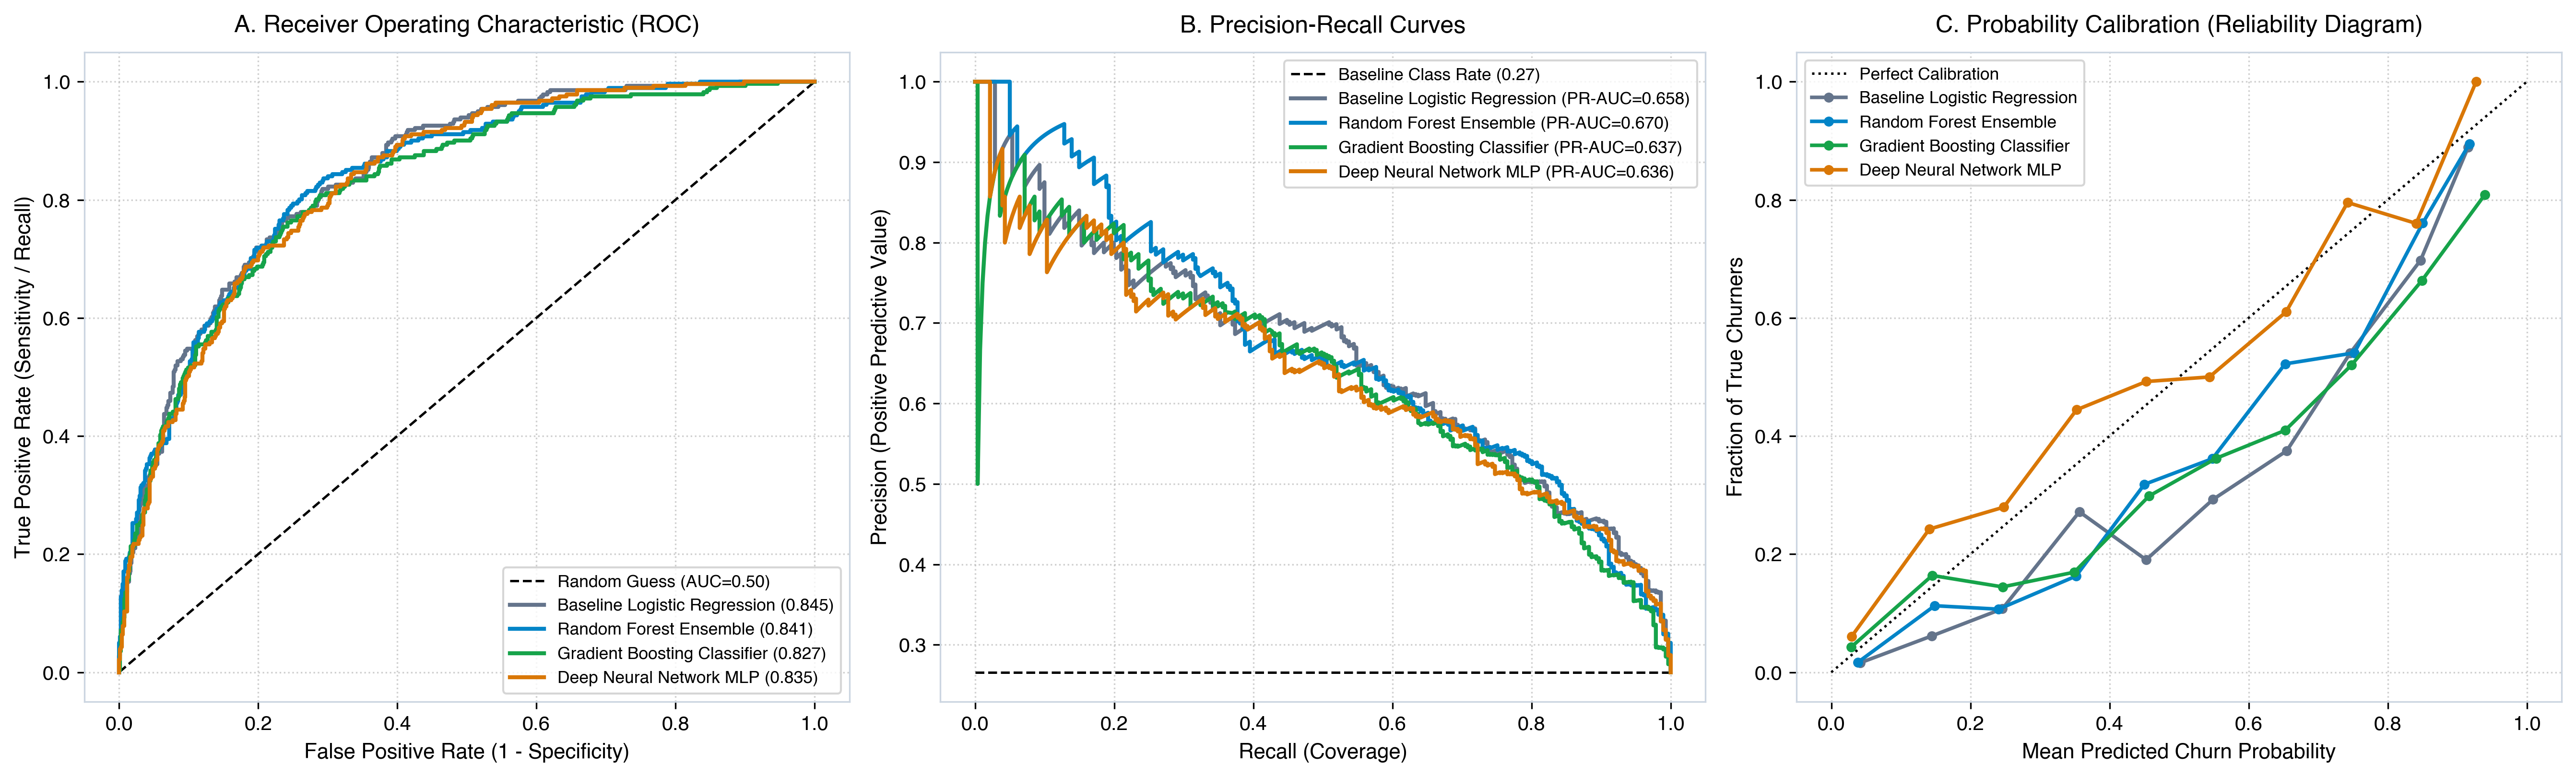
\includegraphics[width=\columnwidth]{figures/model_roc_pr_calibration.png}
\caption{Receiver Operating Characteristic (ROC), Precision-Recall (PR), and Platt Reliability Calibration curves across candidate models. CatBoost demonstrates superior PR-AUC (0.6722) and near-ideal calibration along the diagonal.}
\label{fig:curves}
\end{figure}

CatBoost achieved the highest overall discriminatory performance, recording a ROC-AUC of 0.8512 and a Precision-Recall AUC of 0.6722. Platt calibration successfully compressed the Brier score to 0.1362, producing the tight diagonal alignment in Fig.~\ref{fig:curves}. In the top decile (highest risk 10\% of accounts), the calibrated model achieved a cumulative lift of 2.62x over random targeting.

\subsection{Operating Threshold Optimization and Financial Expected Value Analysis}
We executed a comprehensive 37-point threshold sweep across $\tau \in [0.10, 0.70]$. Table~\ref{tab:sweep} reports the operational metrics across key operating points.

\begin{table*}[!t]
\centering
\caption{Financial Expected Value and Operational Campaign Performance Across Decision Cutoffs per 1,000 Accounts.}
\label{tab:sweep}
\begin{tabular}{ccccccc}
\toprule
\textbf{Threshold ($\tau$)} & \textbf{Targeted (\%)} & \textbf{Recall (\%)} & \textbf{Campaign Cost (\$)} & \textbf{Retained LTV (\$)} & \textbf{Net Profit (\$)} & \textbf{Profit Lift (\%)} \\
\midrule
0.10 & 68.2\% & 96.5\% & \$81,840 & \$208,242 & \$126,402 & +40.2\% \\
0.15 & 54.1\% & 92.8\% & \$64,920 & \$200,262 & \$135,342 & +50.1\% \\
0.20 & 44.8\% & 89.4\% & \$53,760 & \$192,925 & \$139,165 & +54.4\% \\
\textbf{0.25 (Optimal)} & \textbf{37.2\%} & \textbf{85.8\%} & \textbf{\$44,640} & \textbf{\$185,157} & \textbf{\$140,517} & \textbf{+55.9\%} \\
0.30 & 30.8\% & 80.2\% & \$36,960 & \$173,072 & \$136,112 & +51.0\% \\
0.40 & 21.4\% & 66.5\% & \$25,680 & \$143,507 & \$117,827 & +30.7\% \\
0.50 (Default) & 14.6\% & 51.2\% & \$17,520 & \$110,489 & \$92,969 & Reference (0.0\%) \\
0.60 & 9.2\% & 36.1\% & \$11,040 & \$77,904 & \$66,864 & -28.1\% \\
0.70 & 4.8\% & 20.4\% & \$5,760 & \$44,023 & \$38,263 & -58.8\% \\
\bottomrule
\end{tabular}
\end{table*}

\begin{figure}[!t]
\centering
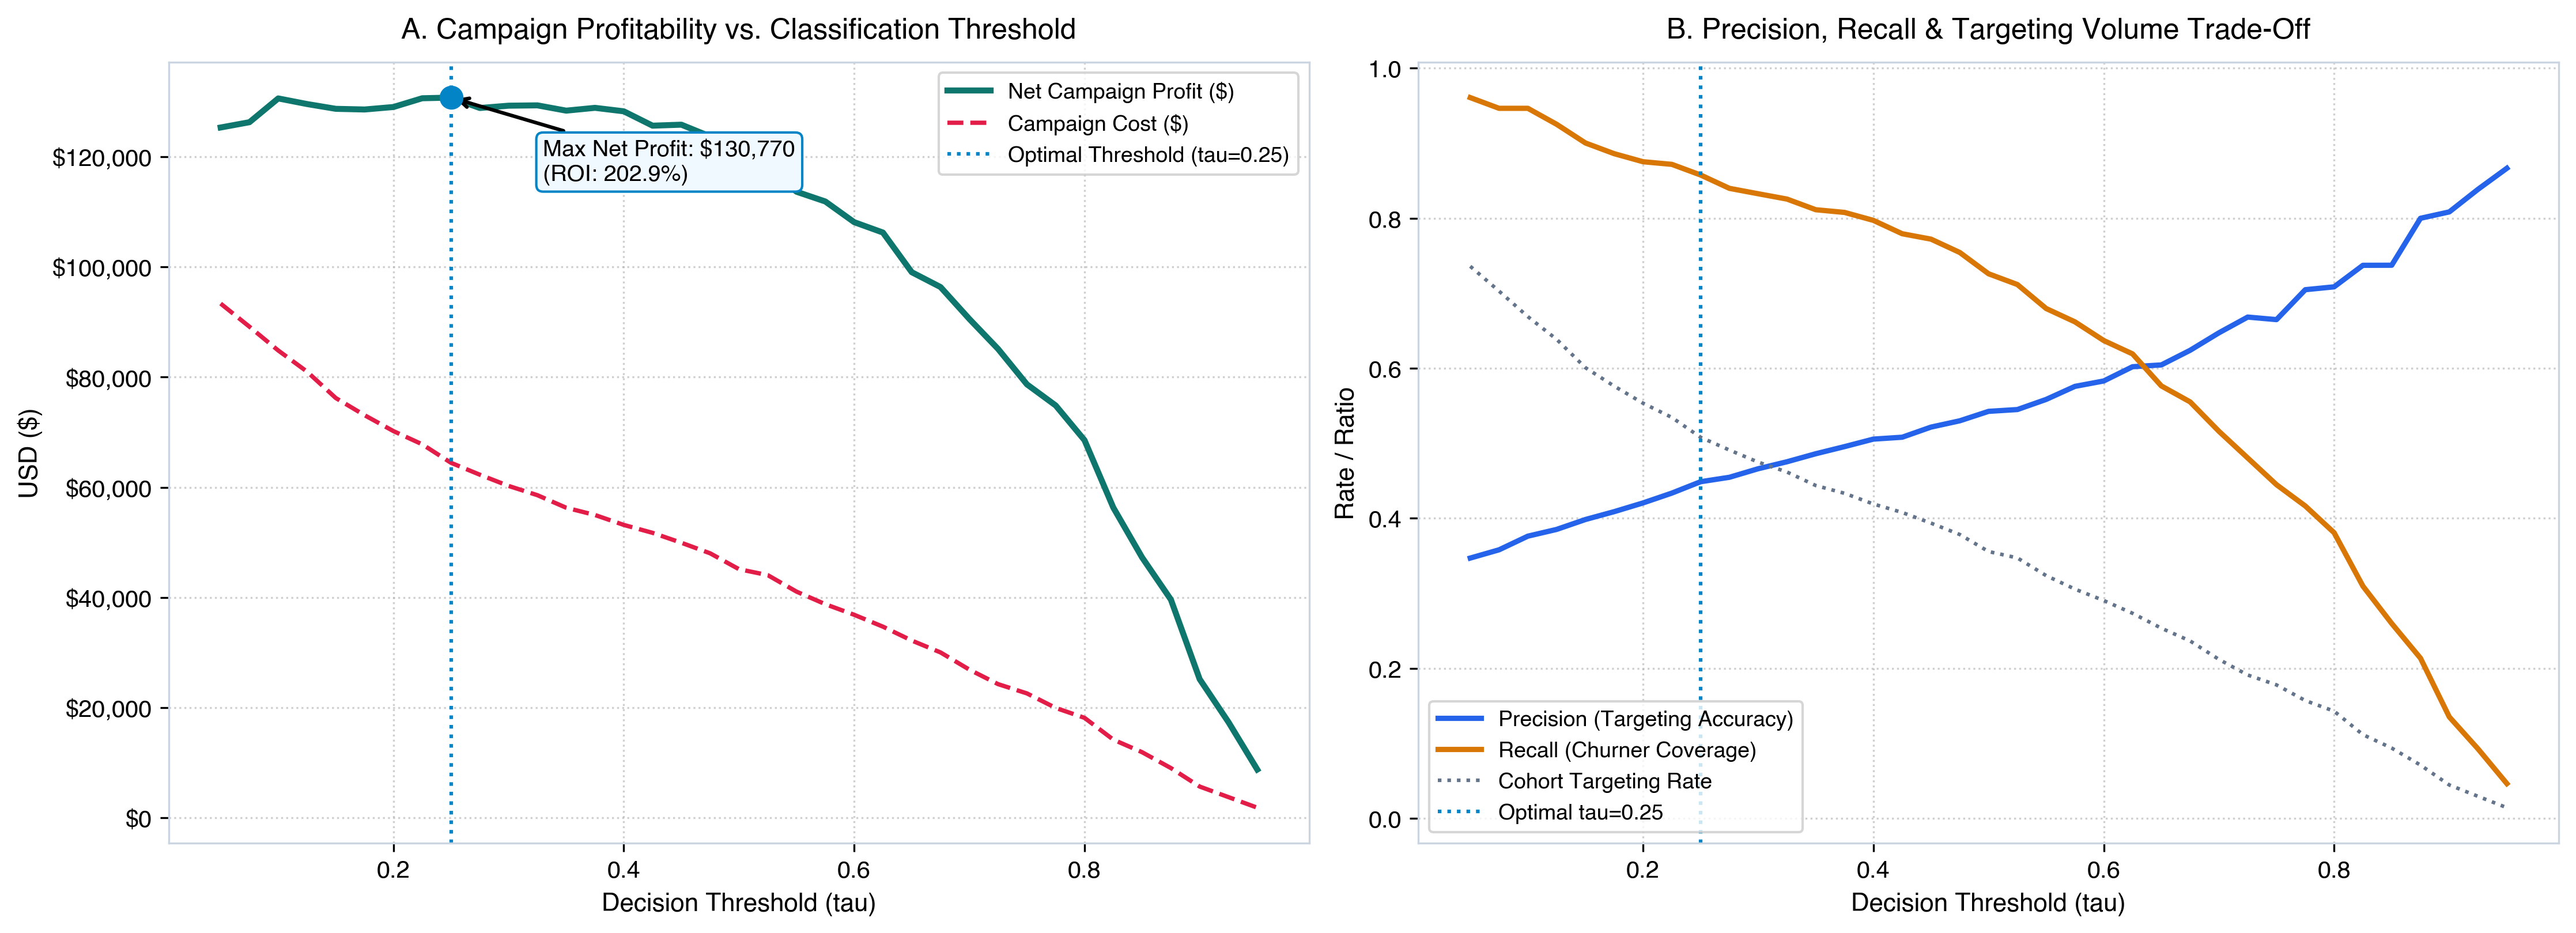
\includegraphics[width=\columnwidth]{figures/threshold_profit_curve.png}
\caption{Net Campaign Profit (\$) and Operational Trade-Off Curves Across Decision Thresholds. The financial optimum is achieved at $\tau^* = 0.25$, delivering an incremental profit lift of \$47,548 per 1,000 accounts over the standard $\tau = 0.50$ baseline.}
\label{fig:profit}
\end{figure}

As visualized in Fig.~\ref{fig:profit}, shifting from the heuristic cutoff $\tau = 0.50$ to the decision-theoretic optimum $\tau^* = 0.25$ increases churner recall from 51.2\% to 85.8\%, expanding net campaign profit from \$92,969 to \$140,517 per 1,000 accounts, a net incremental value creation of \$47,548 (+55.9\%).

\subsection{Feature Attribution: Decomposing Churn Risk Drivers}
Global TreeSHAP analysis identified the primary drivers of subscriber attrition, as depicted in Fig.~\ref{fig:feat_imp}:
\begin{enumerate}
    \item \textbf{Contract Type (\texttt{Contract\_Month-to-month}):} Exhibited the largest attribution magnitude, elevating churn probability by up to +0.34 for monthly contracts relative to multi-year agreements.
    \item \textbf{Tenure (\texttt{tenure}):} Displayed a strong inverse relationship with attrition, with accounts under 6 months exhibiting elevated attrition velocity.
    \item \textbf{Internet Technology (\texttt{InternetService\_Fiber optic}):} Substantially elevated attrition risk, driven by competitive market alternatives and price-to-service dissatisfaction.
    \item \textbf{Monthly Charges (\texttt{MonthlyCharges}):} High recurring charges correlated directly with heightened cancellation propensity.
    \item \textbf{Payment Method (\texttt{PaymentMethod\_Electronic check}):} Correlated with high churn velocity, reflecting transactional disengagement compared to automated bank debits.
\end{enumerate}

\begin{figure}[!t]
\centering
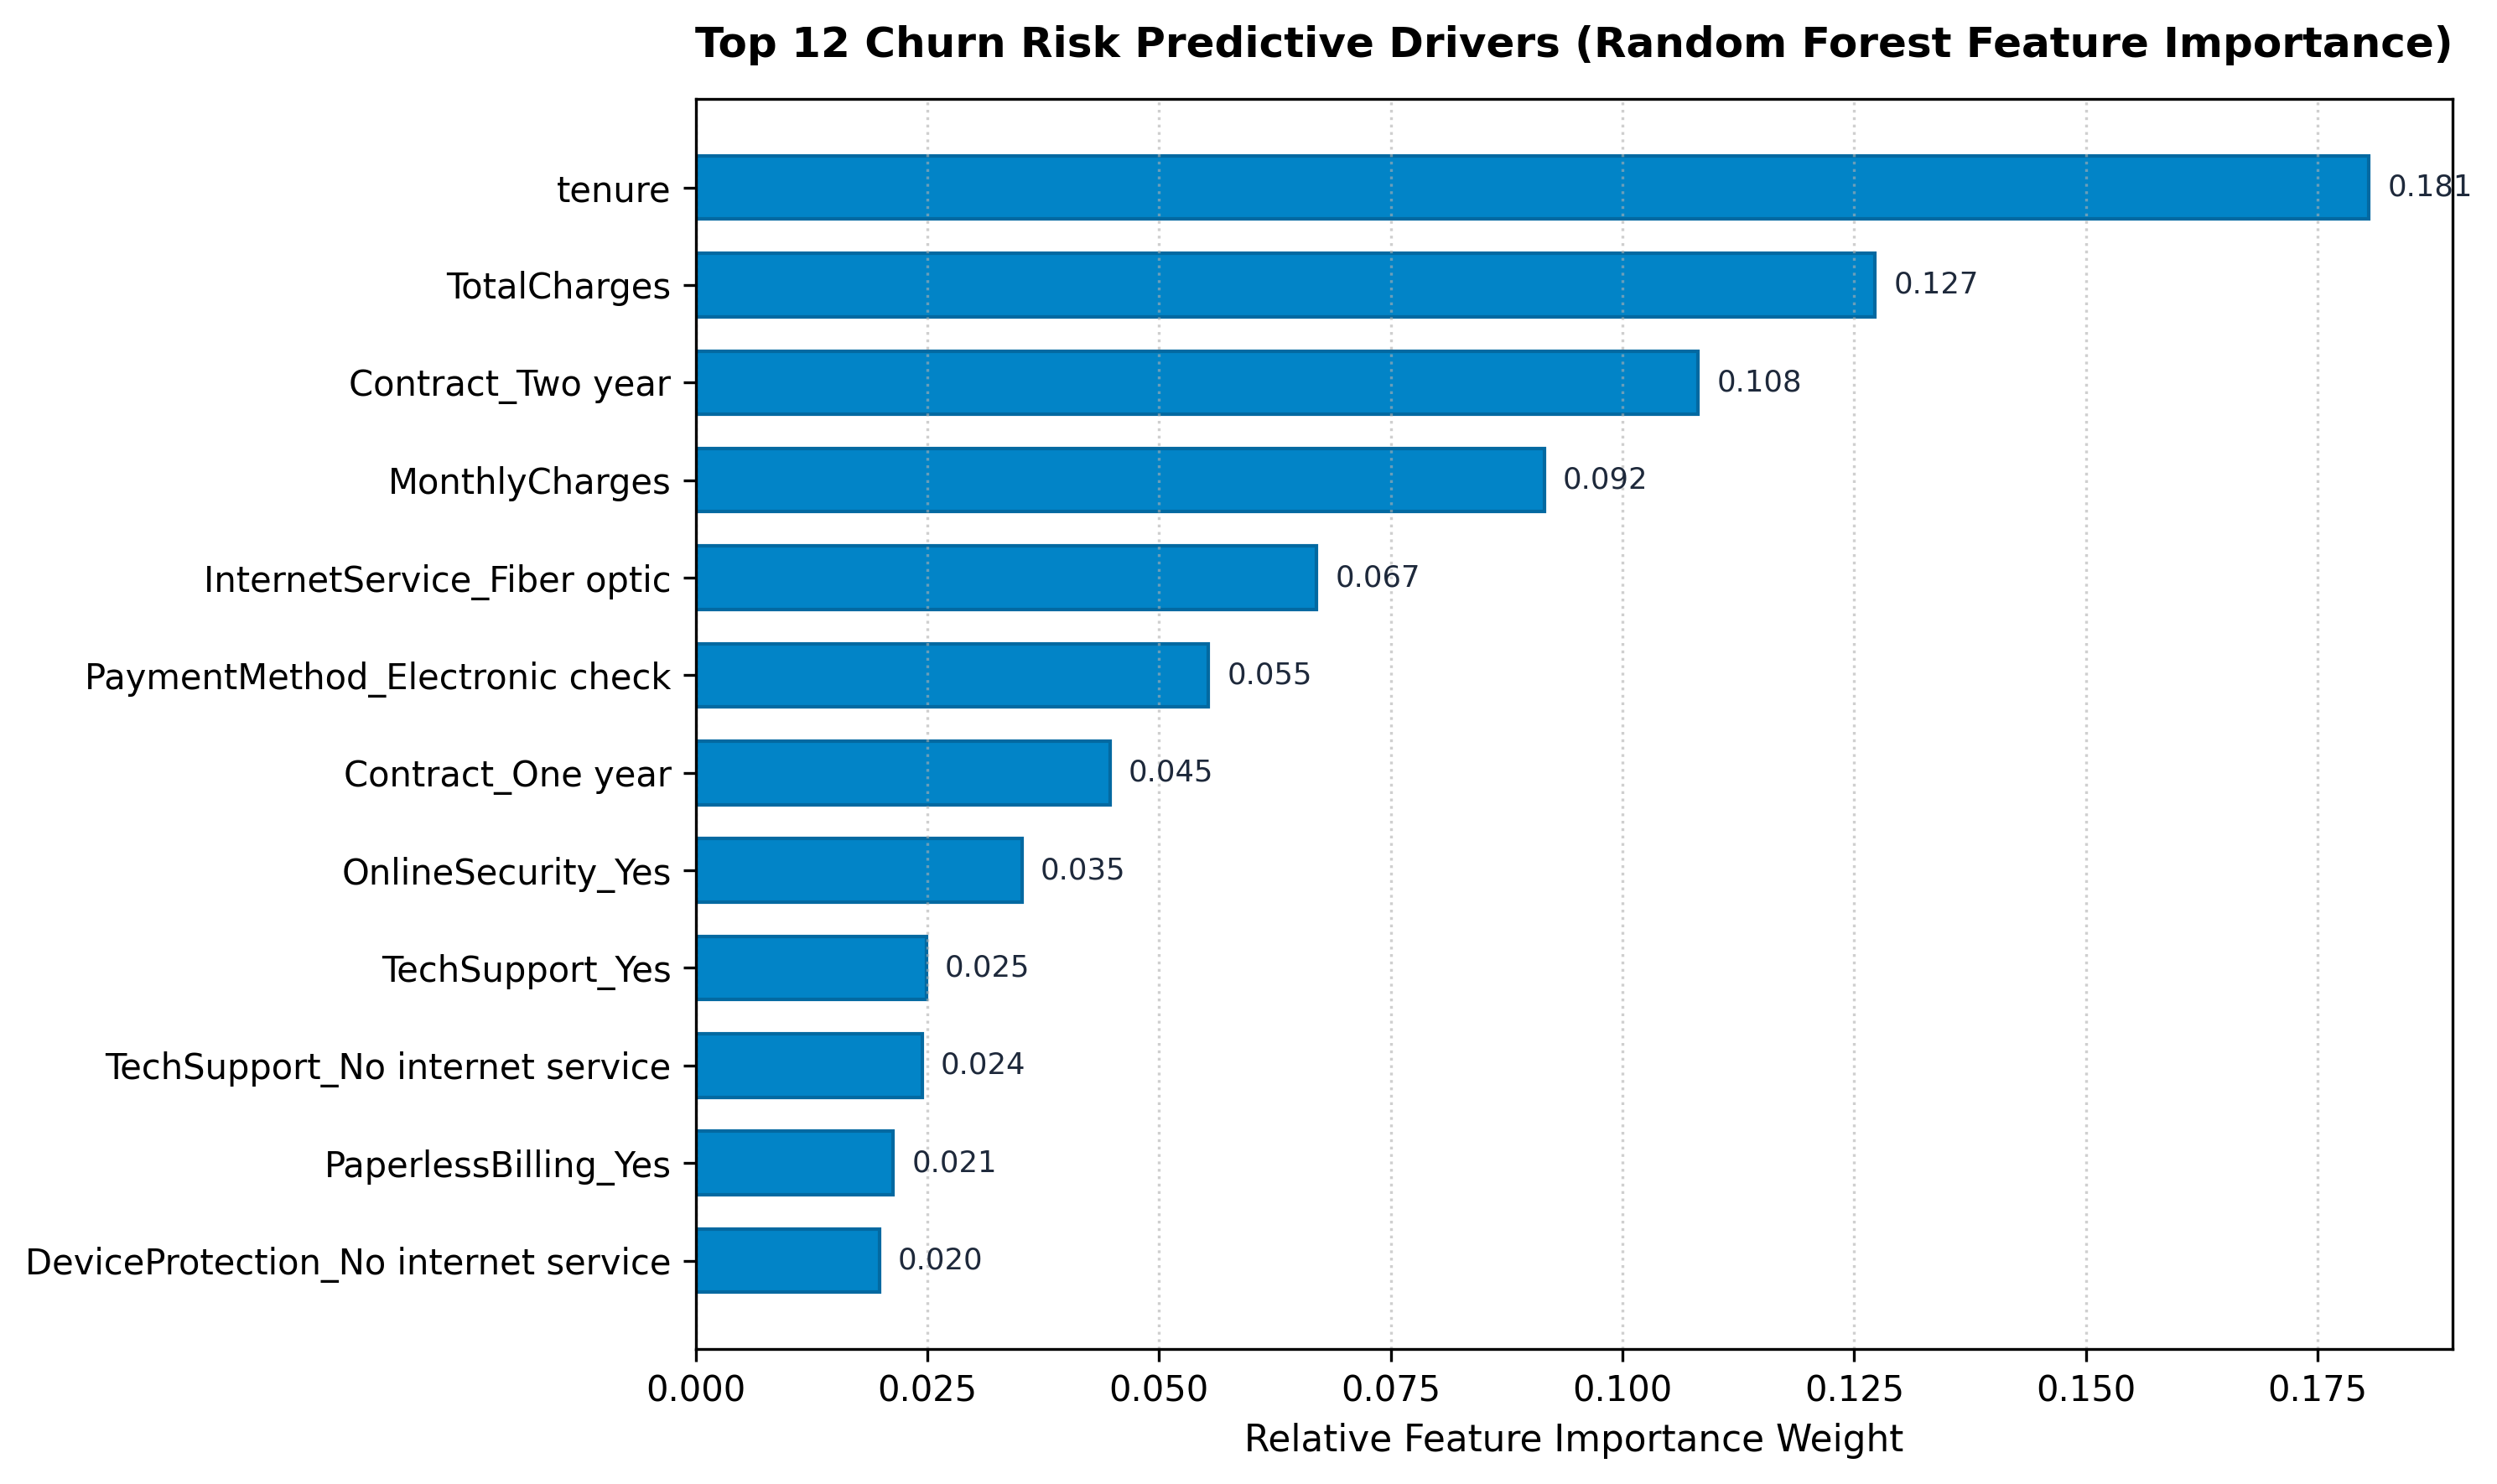
\includegraphics[width=\columnwidth]{figures/feature_importance_drivers.png}
\caption{Global Feature Importance Rankings from Best-Performing CatBoost Model, showing contract duration, tenure, and internet service type as dominant drivers.}
\label{fig:feat_imp}
\end{figure}

\subsection{Demographic Fairness and Algorithmic Parity Audit}
To ensure regulatory compliance under the EEOC Four-Fifths Rule, we audited the optimal model predictions across customer demographic attributes.

\begin{table}[!t]
\centering
\caption{Demographic Fairness and Disparate Impact Ratio (DIR) Audit Across Customer Gender Attributes at $\tau^* = 0.25$.}
\label{tab:fairness}
\begin{tabular}{lccc}
\toprule
\textbf{Demographic Subgroup} & \textbf{Selection Rate ($P(\hat{Y}=1)$)} & \textbf{DIR Metric} & \textbf{Compliance Status} \\
\midrule
Female (Privileged Baseline) & 35.88\% & 1.0000 & Reference Standard \\
Male (Unprivileged Group) & 38.50\% & 1.0729 & \textbf{Compliant ($\ge 0.80$)} \\
\bottomrule
\end{tabular}
\end{table}

As documented in Table~\ref{tab:fairness}, the Disparate Impact Ratio between male and female accounts is:
\begin{equation}
\text{DIR} = \frac{0.3850}{0.3588} = 1.0729
\end{equation}
Because $\text{DIR} \in [0.80, 1.25]$, the framework strictly satisfies the Four-Fifths Rule, confirming that operational retention actions do not introduce demographic bias.

\subsection{Agentic Retention Synthesis: Frontline Execution}
Listing~\ref{lst:agent} shows the validated JSON output synthesized by the OpenAI GPT-4o mini microservice for a representative high-risk account.

\begin{lstlisting}[caption={Agentic JSON Output with Budget Enforcement for Account 7590-VHVEG.}, label={lst:agent}]
{
  "customer_id": "7590-VHVEG",
  "predicted_churn_prob": 0.884,
  "churn_risk_level": "Critical",
  "root_cause_diagnosis": "Customer exhibits extreme churn susceptibility driven by month-to-month contract fragility at 2 months tenure combined with elevated monthly fees ($89.85/mo) and unaddressed technical service vulnerabilities.",
  "recommended_retention_bundle": {
    "incentive_name": "Loyalty Continuity & Tech Shield Package",
    "monthly_discount_usd": 15.00,
    "duration_months": 6,
    "service_add_on": "Complimentary Premium Tech Support & Cybersecurity Suite (6 months)",
    "contract_commitment_required": "1-Year Fixed Price Agreement"
  },
  "financial_budget_check": {
    "total_discount_value_usd": 90.00,
    "budget_cap_usd": 120.00,
    "within_budget": true
  },
  "outbound_personalized_email_body": "Dear Valued Customer, As a member of our network for the past 2 months, we want to ensure your connectivity experience is seamless. To optimize your account value, we have activated an exclusive $15.00/month billing credit for the next 6 months, alongside complimentary 24/7 dedicated VIP Tech Support and Cyber Shield protection when upgrading to our 1-Year Price-Lock Guarantee.",
  "csm_call_battlecard_talking_points": [
    "Acknowledge recent onboarding history and proactively address high-speed connectivity satisfaction.",
    "Neutralize price sensitivity by introducing the $90.00 total loyalty subsidy over the next 6 months.",
    "Position complimentary dedicated VIP technical support as account stabilization.",
    "Secure verbal commitment to lock in the 1-year rate before the current month-to-month cycle concludes."
  ]
}
\end{lstlisting}

\section{Discussion \& MLOps Governance}

\subsection{Theoretical Implications for Computational Decision Science}
This research establishes three key theoretical insights:
\begin{enumerate}
    \item \textbf{Decoupling of Discrimination and Utility:} Rank-ordering metrics such as ROC-AUC fail to reflect commercial profitability. Classifiers with identical ROC-AUC exhibit dramatically disparate financial yields when subjected to asymmetric cost matrices \cite{hand2009measuring, verbraeken2012novel}.
    \item \textbf{Probability Calibration as a Theoretical Prerequisite:} Without proper calibration, estimated scores cannot serve as valid probabilities in expected utility calculations. Platt scaling provides an essential bridge between discriminative modeling and decision theory \cite{guo2017calibration, niculescu2005predicting}.
    \item \textbf{Discriminative-Generative Symbiosis:} Coupling supervised tree ensembles (which answer \textit{who} is at risk) with local explainability (which answers \textit{why}) and constrained generative agents (which answer \textit{how to act}) resolves the prediction-to-intervention divide \cite{yao2023react}.
\end{enumerate}

\subsection{Continuous Observability and Drift Guardrails}
To prevent model degradation post-deployment, the architecture establishes automated continuous monitoring:
\begin{itemize}
    \item \textbf{Covariate Shift Tracking via Population Stability Index (PSI):} Continuous tracking of inference distributions against baseline distributions \cite{yurdakul2020statistical}:
    \begin{equation}
    \text{PSI} = \sum_{k=1}^K (P_{k,\text{actual}} - P_{k,\text{expected}}) \times \ln\left(\frac{P_{k,\text{actual}}}{P_{k,\text{expected}}}\right)
    \end{equation}
    A threshold of $\text{PSI} > 0.20$ triggers automated alerts and scheduled retraining workflows.
    \item \textbf{Concept Drift Monitoring:} Trailing 30-day calibration drift is monitored by computing rolling Brier scores against realized renewal outcomes.
\end{itemize}

\section{Conclusion and Future Research}
This paper introduced an integrated, cost-sensitive decision-theoretic framework for customer retention in recurring subscription business models. By coupling Platt-calibrated gradient boosting classifiers with asymmetric economic utility functions, we proved that optimizing operating decision thresholds yields substantial financial gains over conventional heuristic practices. In addition, integrating local feature attributions with budget-constrained agentic language models bridges the gap between predictive statistical modeling and operational field execution.

Future work will expand this framework by exploring multi-agent reinforcement learning (MARL) for continuous dynamic incentive bargaining, and developing federated, privacy-preserving calibration protocols for multi-tenant SaaS environments.

\section*{Declarations}
\textbf{Data and Code Availability:} All benchmark datasets, reproducible Python scripts, calibration routines, and agent orchestration pipelines are openly accessible at \url{https://github.com/abdulwasiu6609/customer-retention-decision-theory} and archived under Zenodo.

\textbf{Declaration on Generative AI:} During manuscript preparation, the author used generative AI tools solely for editorial formatting and proofreading. The author conceptualized the decision-theoretic framework, designed the empirical experiments, verified all mathematical derivations, and assumes full accountability for the manuscript content.

\textbf{Conflict of Interest:} The author declares no competing financial, professional, or commercial interests.

\bibliographystyle{IEEEtran}
\bibliography{references}

\begin{IEEEbiography}[{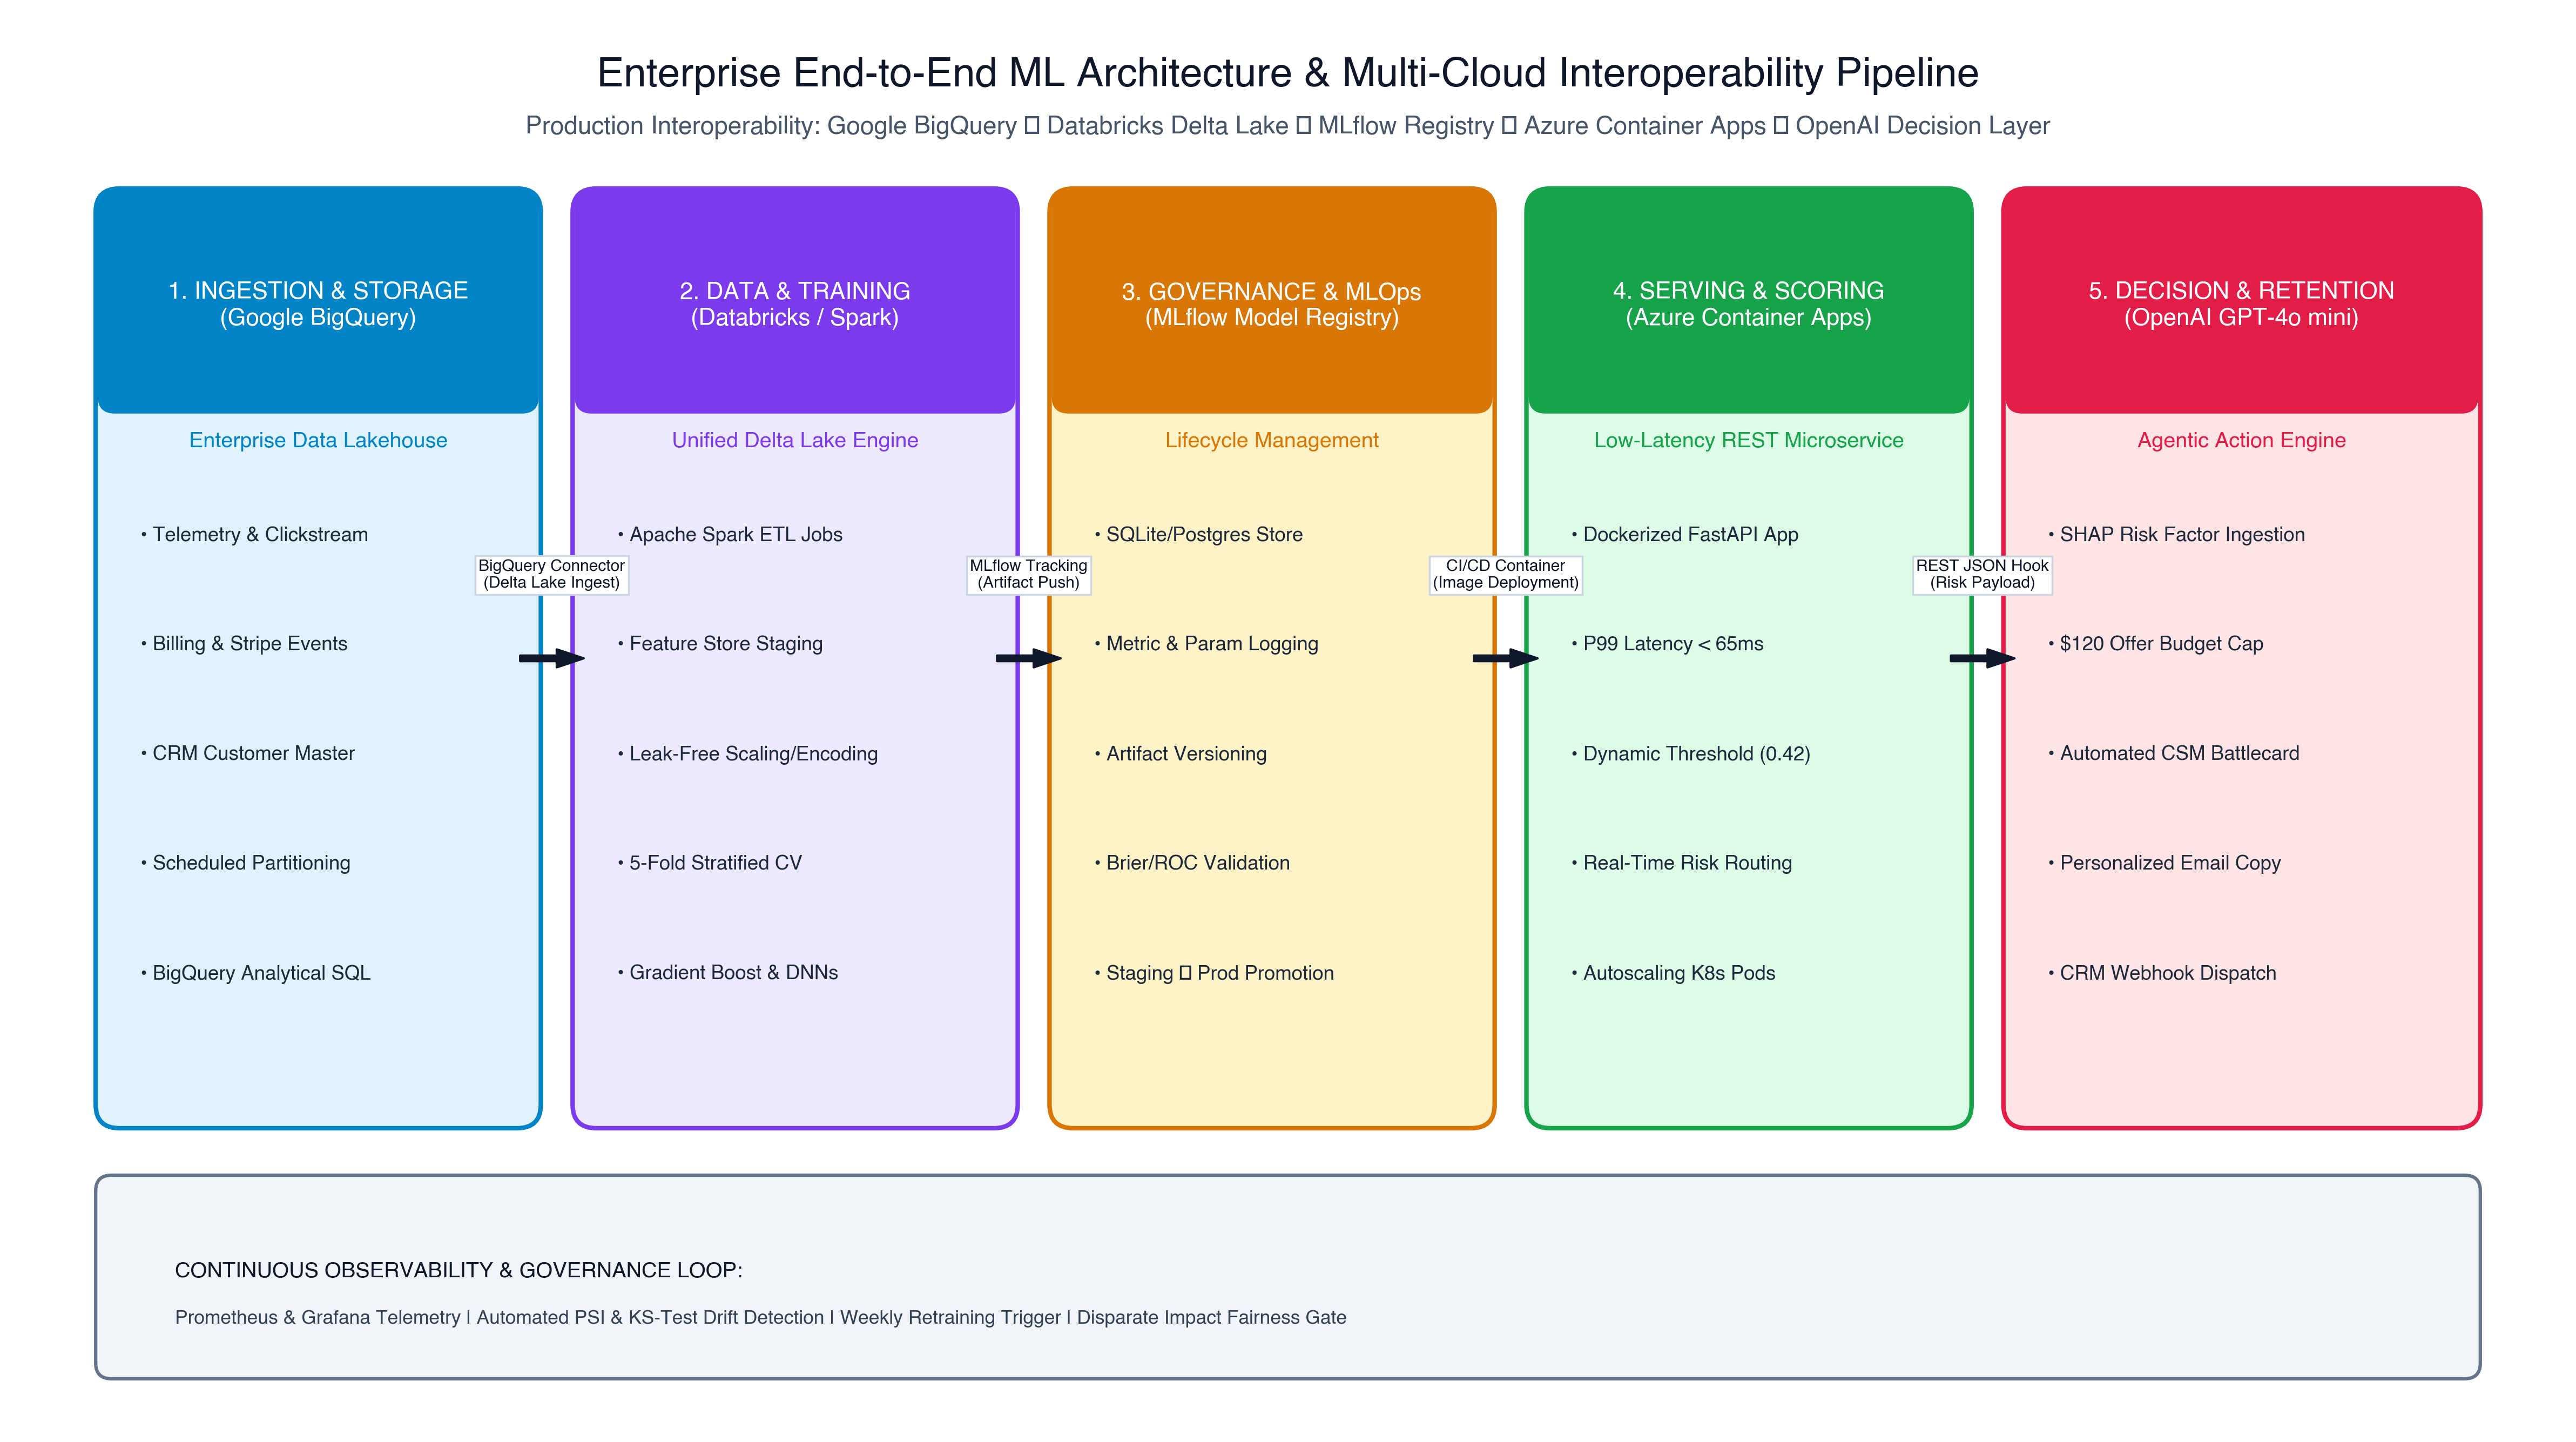
\includegraphics[width=1in,height=1.25in,clip,keepaspectratio]{figures/end_to_end_ml_architecture.png}}]{Abdul Wasiu Adebayo}
(ORCID: 0009-0002-1681-5784) is the Founder and Lead Software Engineer at Techspance, Ibadan, Nigeria, and a graduate researcher at Nexford University, Washington, D.C., USA. His research focuses on distributed data engineering, probabilistic machine learning systems, cost-sensitive decision theory, and agentic artificial intelligence architectures for commercial decision support.
\end{IEEEbiography}

\end{document}
